\documentclass{article}
\usepackage{graphicx} % Required for inserting images
\usepackage{amsmath}
\usepackage{amsfonts}
\usepackage{minted} % For code with syntax highlighting
\usepackage[swedish]{babel}

\title{Raketstyrning}
\author{}
\date{September 2026}

\newcommand{\bfbar}[1]{\ensuremath{\mathbf{\bar{#1}}}}

\begin{document}

\maketitle
\tableofcontents


\newpage
\section{Introduktion}
Detta projekt har som syfte att simulera styrningen av en raket mot ett givet mål. Detta inkluderar dels att lösa den differentialekvation som beskriver raketens bana, samt att hitta en metod för att styra raketen mot målet. Raketen rör sig i två dimensioner och motorerna går alltid på full kraft, så att styra raketen innebär i detta fall att bestämma den vinkel motorn är riktad mot.
\newpage
\section{Matematiska modeller och lösningsmetoder}

Vi utgick från den givna ekvationen
\[
    m(t)\bfbar{a}(t) = \bfbar{F} + m'(t) \bfbar{u}(t)
\]
där
\[
    \begin{aligned}
         & \bfbar{F}    &  & = m(t) \bfbar{g} - c||\bfbar{v}(t)||\bfbar{v}(t) \\
         & m(t)         &  & = \begin{cases}
                                   8 - 0.4t & t \leq 10 \\
                                   4        & t > 10
                               \end{cases}                           \\
         & \bfbar{u}(t) &  & = \begin{pmatrix}
                                   k_m \cos(\theta(t)) \\
                                   k_m \sin(\theta(t))
                               \end{pmatrix}
    \end{aligned}
\]
Ur dessa löses
\[
    \begin{aligned}
         & m'(t)        &  & = \begin{cases}
                                   -0.4 & t < 10 \\
                                   0    & t > 10
                               \end{cases}                                                                    \\
         & \bfbar{a}(t) &  & = \frac{m(t) \bfbar{g} - c||\bfbar{v}(t)||\bfbar{v}(t) + m'(t) \bfbar{u}(t)}{m(t)}
    \end{aligned}
\]
Vi har valt att utöka \(m'(t)\) till att vara definierad på hela \(\mathbb{R}\). Dessutom har vi låtit \(\theta\) även bero på positionen och hastigheten för att få
\[
    \begin{aligned}
         & m'(t)             &  & = \begin{cases}
                                        -0.4 & t \leq 10 \\
                                        0    & t > 10
                                    \end{cases}                                                                                                     \\
         & \bfbar{u}(\theta) &  & = \begin{pmatrix}
                                        k_m \cos(\theta) \\
                                        k_m \sin(\theta)
                                    \end{pmatrix}                                                                                                     \\
         & \bfbar{a}(t)      &  & = \frac{m(t) \bfbar{g} - c||\bfbar{v}(t)||\bfbar{v}(t) + m'(t) \bfbar{u}(\theta(t, \bfbar{p}(t), \bfbar{v}(t)))}{m(t)}
    \end{aligned}
\]
Eftersom vi är intresserade av raketens position över tid noterar vi att \(\bfbar{p}''=\bfbar{v}'=\bfbar{a}\) och att ekvationen för \(\bfbar{a}(t)\) är en andra ordningens ODE. Vi skriver om denna som ett system av första ordningens ODE:er.
\[
    \begin{aligned}
         & y  &  &
        = \begin{pmatrix}
              y_p \\
              y_v
          \end{pmatrix}
        =\begin{pmatrix}
             \bfbar{p}(t) \\
             \bfbar{v}(t)
         \end{pmatrix} \\
         & y' &  &
        = \begin{pmatrix}
              y_p' \\
              y_v'
          \end{pmatrix}
        = \begin{pmatrix}
              \bfbar{p}'(t) \\
              \bfbar{v}'(t)
          \end{pmatrix}
        = \begin{pmatrix}
              \bfbar{v}(t) \\
              \bfbar{a}(t)
          \end{pmatrix}
        = \begin{pmatrix}
              y_v \\
              \frac{m(t) \bfbar{g} - c||y_v||y_v + m'(t) \bfbar{u}(\theta(t, y_p, y_v))}{m(t)}
          \end{pmatrix}
    \end{aligned}
\]
Eftersom begynnelsevärdena är givna kan vi definiera ett \(f(t, y)\) för att applicera kända lösningsmetoder på problemet \(y'=f(t, y)\).
\[
    \begin{aligned}
         & f(t, y) &  & = \begin{pmatrix}
                              y_v \\
                              \frac{m(t) \bfbar{g} - c||y_v||y_v + m'(t) \bfbar{u}(\theta(t, y_p, y_v))}{m(t)}
                          \end{pmatrix} \\
         & y_0     &  & = \begin{pmatrix}
                              \bfbar{p}(0) \\
                              \bfbar{v}(0)
                          \end{pmatrix}
        = \begin{pmatrix}
              \bfbar{0},
              \bfbar{0}
          \end{pmatrix}
    \end{aligned}
\]
ODE:n, och därför lösningen, beror nu fortfarande på funktionen \(\theta\). Givet är att \(\theta = -\frac{\pi}{2}\) innan \(\bfbar{p} \geq 20\) första gången. Vi har valt att definiera ett \(\theta\) som håller en konstant vinkel \(\alpha\) över denna höjd enligt
\[
    \theta(t, \bfbar{p}, \bfbar{v}) = \begin{cases}
        -\frac{\pi}{2} & \bfbar{p} < 20    \\
        \alpha         & \bfbar{p} \geq 20
    \end{cases}
\]
Målet är nu att hitta ett \(\alpha\) så att \(\bfbar{p}(t) = \begin{pmatrix}
    80,
    60
\end{pmatrix}\) för något \(t\). Genom att definiera raketens minsta distans från målet som
\[
    D(\alpha) = \min_{t \geq 0}\left(||y_p - \begin{pmatrix}
            80,
            60
        \end{pmatrix}||\right)
\]
kan vi hitta detta \(\alpha\), och därmed vårat \(\theta\), genom att lösa \(D(\alpha) = 0\).

\newpage

\section{Tolkning och analys}
\begin{figure}[h]
    \begin{center}
        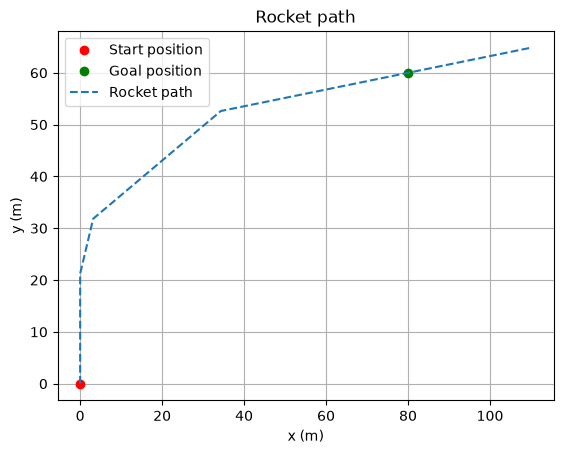
\includegraphics[width=\textwidth]{images/solve_ivp-constant-angle-plot.png}
        \caption{Simulation med solve\_ivp, $\alpha=-3.02$}
        \label{fig:solve-ivp}
    \end{center}
\end{figure}

\begin{figure}[h]
    \begin{center}
        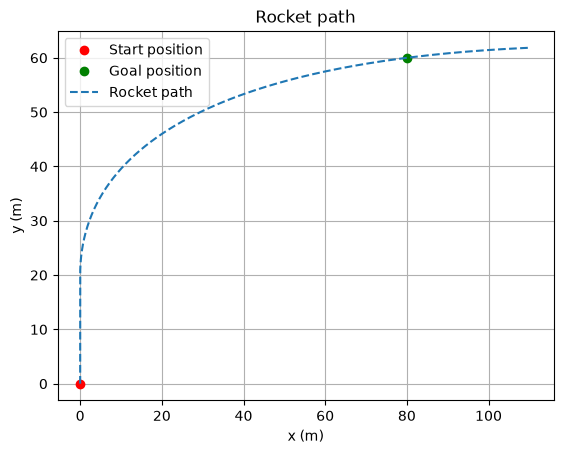
\includegraphics[width=\textwidth]{images/rk4-constant-angle-plot.png}
        \caption{Simulation med rk4, $\alpha=-3.05$, $h=0.01$}
        \label{fig:rk4}
    \end{center}
\end{figure}

Vid körningar av modellen har raketen massan 4 kg, luftmotståndskoefficienten $c = 0.05 kg/m$, och raketmotorns hastighet är $k_m = 700 m/s$. Körning av fsolve för att hitta konstanta vinkeln $\alpha$ med solve\_ivp som ODE-lösare gav en vinkel $\alpha\approx-3.02$. Vid körning med rk4 med $h=0.01$ som lösare ger istället vinkeln $\alpha\approx-3.05$ se figurer \ref{fig:solve-ivp}, \ref{fig:rk4} för raketens bana vid körningar med de två metoderna och dess beräknade vinklar.

Båda lösarna ger en vinkel $\alpha\approx-3$. Denna vinkel innebär den vinkel som raketmotorerna ska vara vinklade under färden. Alltså visar resultatet vid dessa körningar på att raketmotorerna ska vinklas nästan vinkelrätt mot marken för att nå målet i (80,60). I figurerna ovan går det att se hur raketenerna rör sig under färden, raketen färdas först rakt upp tills $y=20$ för att sedan svänga med en konstant vinkel mot och passerar till slut målet. Vi kan se att solve\_ivp använder ett större tidssteg, vilket beror på att det är en adaptiv metod som väljer ett h som uppfyller en viss feltolerans.




\appendix
\clearpage
\section{Källkod}
\inputminted{python3}{main.py}

\end{document}
